\documentclass{sig-alternate-05-2015}
\newcommand{\showComments}{yes} %% yes or no
\usepackage{xcolor}
\usepackage[hyphenbreaks]{breakurl}
\usepackage[numbers,sort&compress]{natbib}
\usepackage[ruled,vlined,linesnumbered]{algorithm2e}
\usepackage{amssymb}
\usepackage{nicefrac}
\usepackage{setspace}
\usepackage{amsmath}

\setstretch{1.2}
\usepackage[
    breaklinks,
    colorlinks,
    pdfpagelabels=false,
    linkcolor=blue!50!black,
    citecolor=blue!50!black,
    filecolor=blue!50!black,
    urlcolor=blue!50!black,
    draft                       % fixed \pdfendlink bug
  ]{hyperref}
\usepackage{shortcuts}

\def\sharedaffiliation{%
\end{tabular}
\begin{tabular}{c}}


\begin{document}
\setcopyright{acmcopyright}
\title{Virtualized Environment Detection and Mitigation}
%   {IS632: Final Project Report}
\numberofauthors{3}
\author{
  \alignauthor Markus Faerevaag
%
  \alignauthor Jungsuk Oh
%
  \alignauthor Ji Hyeon Yoon
%
  \sharedaffiliation
  \affaddr{{\normalsize \helveticafont School of Computing}}\\
  \affaddr{{\normalsize \helveticafont KAIST}}\\
  \affaddr{{\normalsize \helveticafont Daejeon, Korea}}\\
  {\normalsize \tt \{mfaerevaag, jsoh921, jihyeon.yoon\}@kaist.ac.kr}
}
\maketitle

\begin{abstract}
\begin{abstract}
abstract will be here

\end{abstract}
\end{abstract}

\vspace{8pt}
\section{Introduction}
\label{sec:intro}
Malwares are often analyzed in virtual machines (a.k.a. sandbox) for efficiency. However, sophisticated malwares are able to detect whether it is being executed on virtual machines or real hardware. If it is not on bare metal, then it holds back its malicious activities to hinder the analysis. In CCS\textquotesingle 08, Ether \cite{ether} has introduced a transparent malware analysis method. Three years lalter, P{\'e}k \textit{et al.}\cite{nether} published that Ether\cite{ether} was still detectable by using timing information, CPUID, and CPU errata. Although the fight between malware authors and security researchers on detecting and hiding virtual environment is an ongoing battle, achieving transparency is fundamentally more difficult~\cite{garfinkel2007}.
There are two types of virtualization in general. The first is software based where the guest OS runs on top of a host OS like the VMware or VirtualBox. The second is hardware based virtualization that runs without any host OS but on top of a hypervisor like Intel VT-x. The software based solution is far from perfect. It has countless bugs that it is infeasible to expect transparency. Although the hardware solution is much more stable, clever techniques such as testing the CPU cache remains to be a challenge for the security community.
In this paper we explore how nEther\cite{nether} has broken Ether\cite{ether} and potential mitigation methods for Ether. Our contributions are:

\begin{itemize}
\item We have surveyed Ether\cite{ether} detection techniques used by malware authors
\item We have proposed two novel mitigation method on Ether detection through CPU errata
\item We have emphasized analysis of sophisticated VMs should never be done on software based VM due to their numerous defects 
\end{itemize}

%%% Local Variables:
%%% mode: latex
%%% TeX-master: "../paper"
%%% End:


\vspace{8pt}
\section{Related Work}
\label{sec:related}
\subsection{Ether}
Ether~\cite{ether} is a malware analysis platform that utilizes 
Intel VT's hardware virtualization extensions, and theoretically it has no presence 
in the guest operating system. It uses native CPU instructions, thus does not suffer from 
incomplete or inaccurate system emulation such as hardware emulators do. 
Ether also comes with a rich feature set, thus it can monitor 
all the memory write attempts of the guest, trace the instructions and 
system calls of in-guest processes, and unpack a wide range of protected binaries. 
As a result, malware cannot detect the presence of Ether. In that paper, 
they evaluated Ether and several other state-of-the-art analyzers on the obfuscation techniques 
used to obfuscate 25,000 recent malware samples. The results show that Ether remains transparent 
and defeats the obfuscation tools that evade the existing approaches. 
Ether's system architecture is represented in Figure~\ref{fig:ether} below.

\begin{figure}[!h]
	\centering
	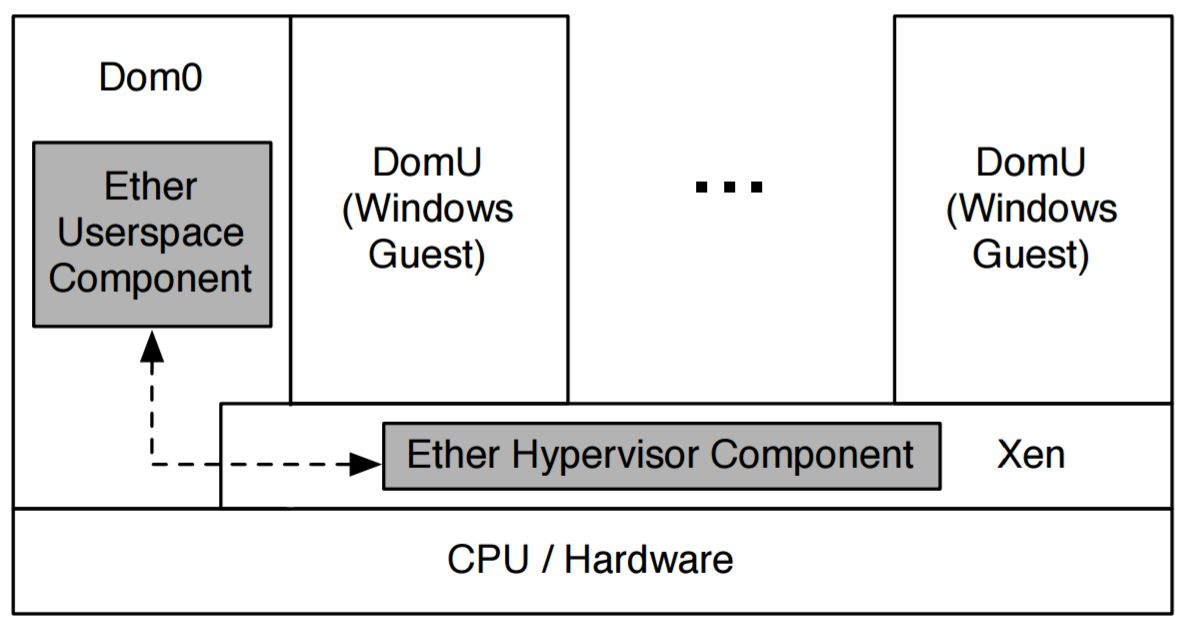
\includegraphics[width=\linewidth]{figure/ether.png}
	\caption{Ether's system architecture.}
	\label{fig:ether}
\end{figure}

\subsection{nEther}
P{\'e}k \textit{et al.} introduced novel approaches that make the detection of 
hardware assisted virtualization platforms and out-of-the-guest 
malware analysis frameworks possible~\cite{nether}. In order to demonstrate their concepts, 
they implemented a scalable and flexible application framework over Window XP 
called \textit{nEther} which can practically disclose the presence of both 
\textit{Ether}~\cite{ether}, and Intel VT by executing multiple feature tests. 
The system overview of nEther is depicted in Figure~\ref{fig:nether} and 
their proposed feature tests consist of three parts as follows: 1) timing information, 
2) CPUID information, and 3) CPU Errata. 

The use of timing information is a well-known techinique to detect the presence 
of traditional debuggers. The simplest way to get timing information is 
the use of internal timers and periodic interrupt sources such as the Time-Stamp Counter(TSC), 
Periodic Interrupt Timper (PIT), and so on. In case of out-of-the-guest malware analyser, 
it falsify internal timers in order to fool a timing test and provide transparency. 
However, the correct manipulation of timing cannot be guaranteed in all the circumstances. 
As a result, nEther can detect the existence of Ether, based on a contradiction 
raised by clock cycle manipulation where the analyzer returns an adjusted cycle 
difference to hide its presence.

The CPUID instruction returns processor identification and feature information 
depending on the content of general registers EAX and ECX. These could be exploited 
by anlyzer detectors as various modifications of the system can be retrieved. 
In case of Ether, it does alter a few bits of information that could be returned 
by the correct configuration of CPUID. Therefore, nEther can detect Ether 
by checking a few bits returned by a CPUID that are specific to Ether.

CPU Errata refer to the collection of design defects or errors and 
it strongly depends on CPU models. nEther exploits bugs in the Core 2 Duo family, 
called AH4 Erratum which unintendedly updates the Last Exception Recored(LER) MSR. 
This errata is not implemented in hardware-assisted-virtualization solutions, such as Xen. 
In other words, this bug will not happen in the hardware-assisted-virtualized runtime environment, 
and as a result, nEther can distinguish virtualized environment from native 
by executing CPU errata and checking whether LER MSR is unexpectedly updated or not. 
These type of feature tests could not reveal the presence of Ether, 
but could reveal the hardware-assisted-virtualized runtime environment. 

\begin{figure}[!h]
	\centering
	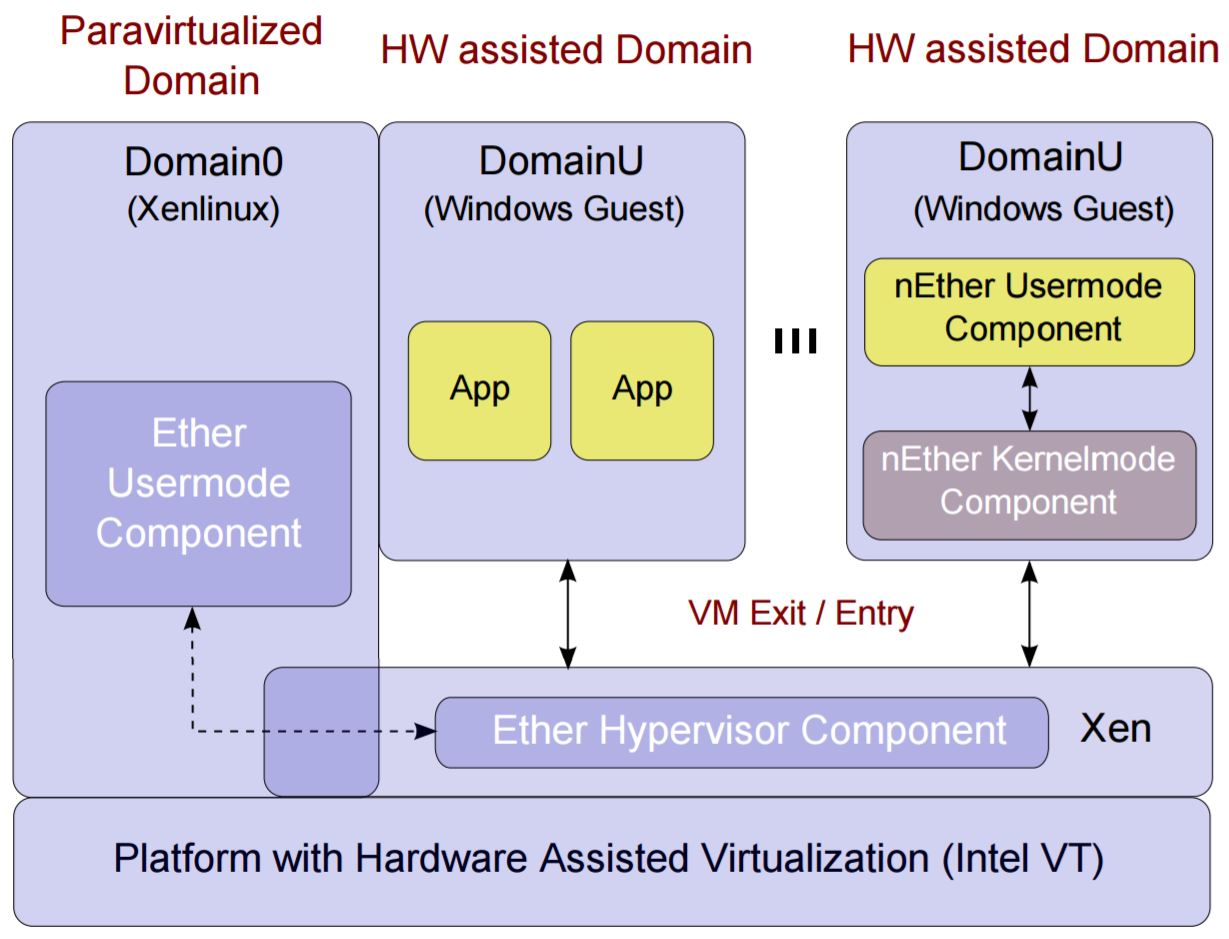
\includegraphics[width=\linewidth]{figure/nether.png}
	\caption{nEther's system overview.}
	\label{fig:nether}
\end{figure}

\subsection{Detecting Virtualized Environment}
Raffetseder \textit{et al.} proposed approaches to identify a processor 
using CPU errata~\cite{raffetseder2007} and it is also valid for detecting system monitors. 
They exploits \textit{Errata N 5} and \textit{Errata N 86} of Intel Pentium 4 processor, 
that result in a segment fault or an incorrect debug exception respectively. 
In QEMU, However, both of errata do not happen or happen differently from native environment. 
As a result, they can detect system monitors, but this is only valid for QEMU hardware emulator.

Several efforts has been made on how relative difference in execution time of
two instructions could be used to detect a virtualized
environment~\cite{raffetseder2007, thompson}. Using absolute time differences is
not feasible, as architectures are complex and different, but the relative
difference is more predictable. Comparing one instruction that is known not to
be trapped by the VMM and one that is, for instance {\tt NOP} and {\tt CPUID}
the authors showed that different VMMs showed significantly different ratios
compared to bare metal.

Ferrie \textit{et al.} showed in 2007 how~\cite{ferrie2007} context switches between an
VMM and guest could be used to detect hypervisors based on Intel VT-x though the
flushing of the Translation Lookaside Buffer (TLB). Using a non-privileged
instruction that is still trapped by the VMM, i.e. {\tt CPUID}, will cause a
flush of the TLB. This could be detected through timing the instruction before
and after anticipated flush. This method has later been documented by other
authors~\cite{thompson}.

Franklin \textit{et al.} proposed an approach to detect VMM by exploiting the timing dependency exception property of a virtual machine monitor~\cite{franklin2008}. Thier approach can detect several different VMMs across the Internet, including VMware and the Xen VMM on a machine with hardware assistance for virtualization.

There are several attempts to defeat detection of virtualized environment. 
Kang \textit{et al.} proposed an approach to dynamically modify the execution of 
a whole-system emulator in order to fool a malware and frustrate anti-emulation techniques 
of malware~\cite{kang2009}. Their approach uses a scalable trace matching algorithm to locate 
the point where emulated execution diverges, and then compares the states of the reference system 
and the emulator to create a dynamic state modification that repairs the difference. 



%%% Local Variables:
%%% mode: latex
%%% TeX-master: "../paper"
%%% End:


\vspace{8pt}
\section{Approach}
\label{sec:approach}
nEther\cite{nether} points out three attack vectors on Ether\cite{ether}: CPUID, CPU errata, and timing information. In this section, we will discuss each attacks and propose our suggested mitigation methods.


\subsection{CPUID Instruction}
\label{sec:approach-cpuid}

Ether alters the output of {\tt CPUID}, flipping the bit for TSC support. Should
be 1 in both VMM and bare metal environment. Can easily be checked, as shown in
Figure~\ref{fig:cpuid-tsc}, in the Appendix.

If it is a bug in the Ether implementation, best solution is to fix, though we
do not have good enough knowledge of the source code to know.

Alternatively, spoof the value in the same manner as {\tt PUSHF} and {\tt POPF}.
Ether deliberately changes the flag register when running, as it sets the debug
flag to be able to step through the target program and get a program trace. It
hides this from the target by spoofing the values of instructions used to read
and write these flags, as {\tt PUSHF} and {\tt POPF}. Figure~\ref{fig:pushf}
shows how the Xen hypervisor is patched to check for specific instructions and
alter the effect of that instruction. The exact same technique could be used to
spoof the TSC-bit when program executes CPUID.

This technique of spoofing the CPUID output suffers from timing attacks, which
will be elaborated in~\nameref{sec:approach-timing}.

\begin{figure}
\begin{lstc}
void vmx_set_pending_exceptions(struct vcpu *v)
{
    ...
+    if(instruction[0] == 0x9C)
+    {
+         /* detected PUSHF */
+
+         v->domain->arch.hvm_domain.ether_controls.send_guest_exception = 1;
+         v->domain->arch.hvm_domain.ether_controls.next_expected_rip = guest_rip + 1;
+    }
+    else if (instruction[0] == 0x9D)
+    {
+         /* detected POPF */
+         ...
+    }
    ...
}
\end{lstc}
\caption{\label{fig:pushf} Part of the patch Ether does on the }
\end{figure}

\subsection{CPU Errata}
\label{sec:approach-errata}
CPU errata refer to the collection of design defects or errors that may induce the CPU to behave differently from the published specification. Such CPU errata is strongly bound to CPU models and nEther exploits bugs in the Core 2 Duo family, called AH4 Erratum. The AH4 Erratum states that "\texttt{VERW/VERR/LSL/LAR} instructions may unexpectedly update the Last Exception Record(LER) MSR" and there is no planned fix for it. Concretely, \texttt{VERW} and \texttt{VERR} instructions verify whether the code or data segment specified with the source operand is readable (\texttt{VERR}) or writable (\texttt{VERW}) from the current privilege level. The \texttt{LAR} instruction loads access rights from a segment descriptor into a general purpose register, and the \texttt{LSL} instruction loads the unscrambled segment limit from the segment descriptor into a general-purpose register~\cite{intelsys}. This erratum is a design fault so its existence is unintended. Therefore, hardware-assisted-virtualization solutions (e.g., Xen) will not implement this erratum in the virtual CPUs of guests, because there is no need to mimic even unexpected system bugs. As a result, malware can detect hardware-assisted virtualization environment by executing those buggy instructions and checking whether LER MSR is unexpectedly updated or not. In other words, this attack cannot recognize the presence of Ether, but can reveal the hardware-virtualized runtime environment. \\

The naive solutions are patching the buggy instructions or use another CPU. However, since they are both infeasible we propose two potential solutions.

\begin{figure}[!h]
	\centering
	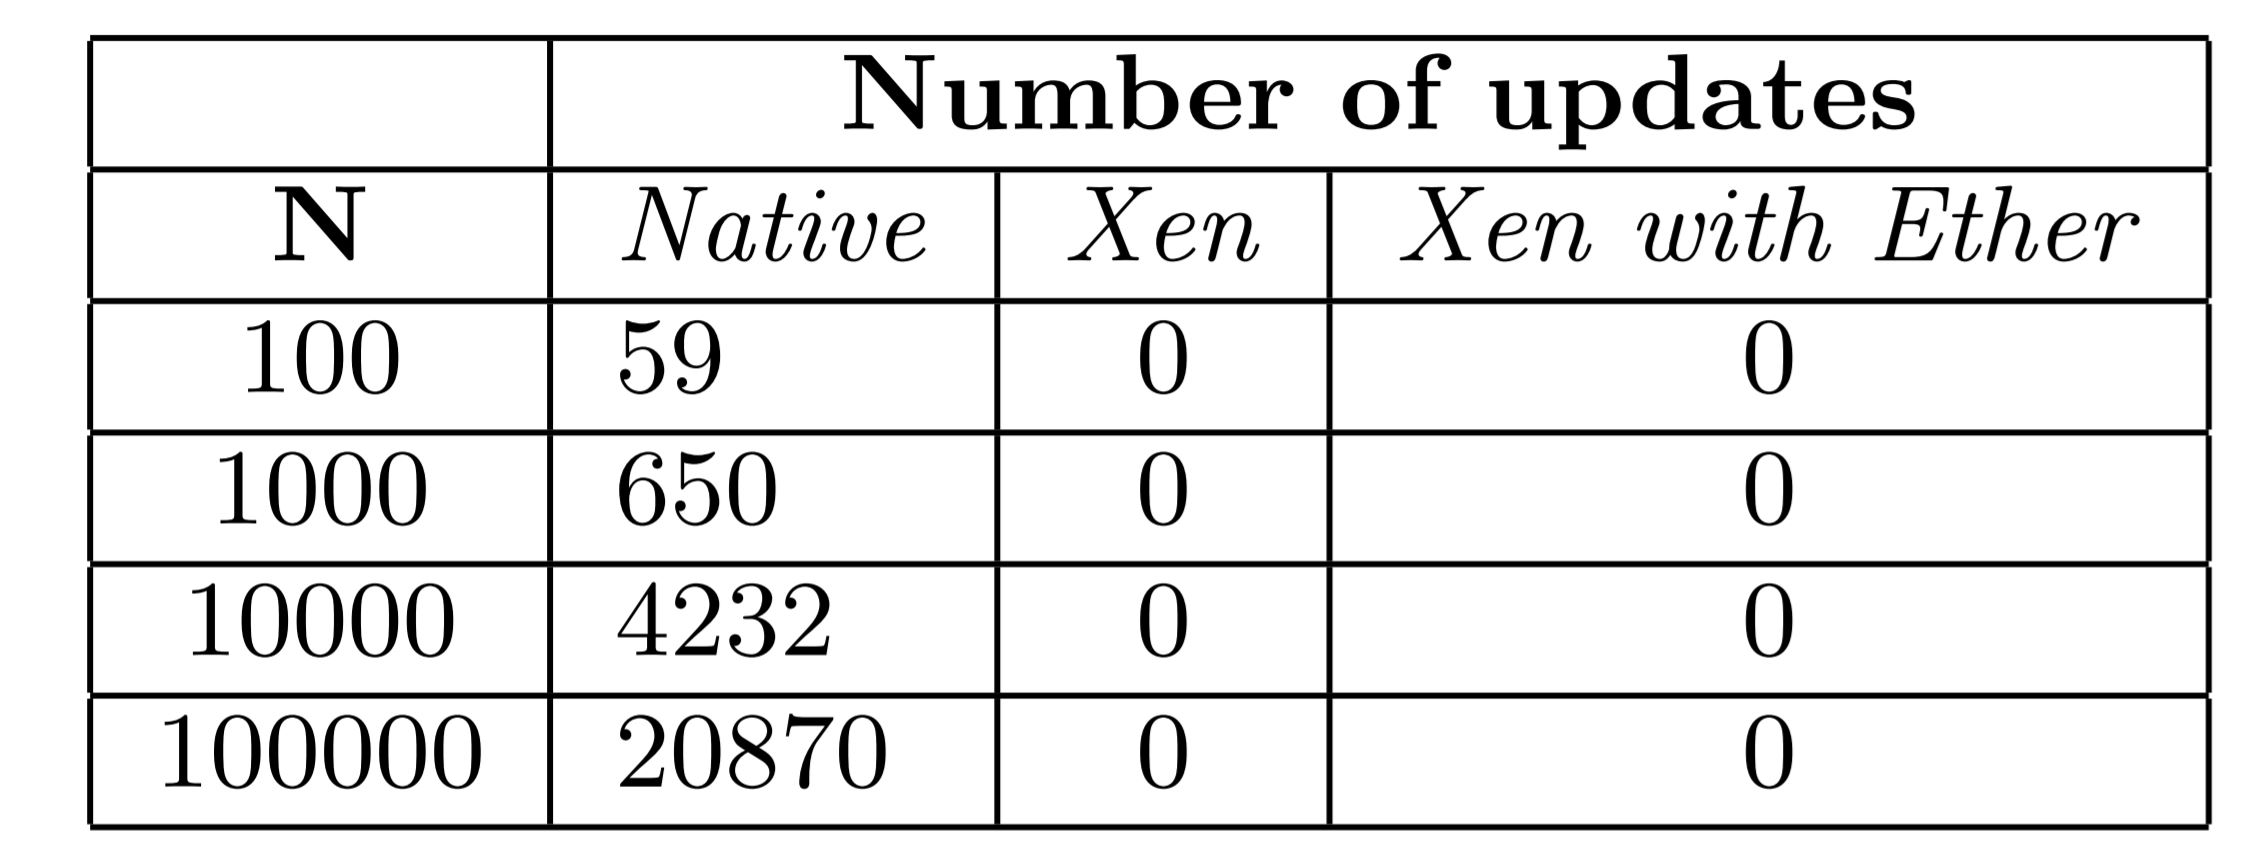
\includegraphics[width=\linewidth]{figure/errata_table.png}
	\caption{The number of LER MSR updates according to the erratum execution}
	\label{fig:errata}
\end{figure}

\subsubsection{Proposed Mitigation 1}
In general, those bugs do not happen always. Table~\ref{fig:errata} demonstrates the number of LER MSR updates when the CPU erratum was executed 100, 1000, 10000 and 100000 times under the corresponding environments. The update occurs only in the native environment, but the frequency of occurrence is unpredictable and irregular(from 20\% up to 65\%). Therefore, this CPU erratum should be executed in several times in order to detect hardware-assisted virtualization environment and this can be considered as a malicious behavior. So, to mitigate this attack, we set the threshold first and then count the number of all execution about those buggy instructions during the runtime of each program. If the counted number exceed the threshold, we can classify that program as a malware or just block to execute buggy instructions anymore. This method cannot prevent from CPU errata attack but can mitigate it, and there is a trade-off between TP and FP depending on how the threshold is set. Note that only kernel mode operations can access to LER MSR, therefore user mode operations does not need to be blocked or classified as a malware, even if execute the CPU erratum unlimited.

\subsubsection{Proposed Mitigation 2}
Another proposed mitigation is to mimic the CPU erratum intentionally. Our goal is to make it difficult to distinguish hardware-virtualized-environment from native one, and the attack exploits that LER MSR update happens only in native environment. Therefore, we may mitigate this attack by updating LER MSR intentionally whenever buggy instructions(\texttt{VERW/VERR/LSL/LAR}) are executed. This method can be implemented in two ways. The first one is to update LER MSR directly right after buggy instructions are executed while monitoring every kernel mode instructions. Note that we do not need to monitor user mode instructions, since attack code should be executed in kernel mode in order to read LER MSR and check whether it is updated or not. The second one is to add LER MSR update code right after every buggy instructions using binary rewriting. LER MSR is divided into {\tt MSR\_LER\_FROM\_LIP} and {\tt MSR\_LER\_TO\_LIP}, and those are located in {\tt 0x1dd} and {\tt 0x1de}, respectively. Therefore, we can add code to modify the value of {\tt0x1dd} and {\tt 0x1de} immediately after \texttt{VERW/VERR/LSL/LAR} instructions, as shown in the Figure~\ref{fig:wrmsr}. Such binary rewriting may be conducted only when kernel module is loaded in the memory in order to minimize performance overhead. This mitigation cannot be applied to self-modifying code, but it is out of scope in our paper.


\begin{figure}[h]
\begin{lstc}
__asm__ {
	/* wrmsr : MSR[ECX] = EDX:EAX; */
	...
	verr ax
+	/* store arbitary value in eax, edx */
+	mov ecx, 0x1dd
+	wrmsr 
+	mov ecx, 0x1de
+	wrmsr
	...
	verw cx
+	/* store arbitary value in eax, edx */
+	mov ecx, 0x1dd
+	wrmsr
+	mov ecx, 0x1de
+	wrmsr
	...
}

\end{lstc}
\caption{\label{fig:wrmsr} Code snippet in assembly showing how to rewrite binary for updating LER MSR intendedly. }
\end{figure}

\subsection{Timing Information}
\label{sec:approach-timing}
Taking advantage of the performance measures and timing information is more sophisticated method for malwares to detect its environment. Although virtual machine\textquotesingle s performance will always slower than it would have been on real hardware, blindly measuring the absolute performance scores is not sufficient to detect virtual environments.\cite{raffetseder2007} Generally, two approaches to use timing information.

\begin{figure*}[!t]
	\centering
	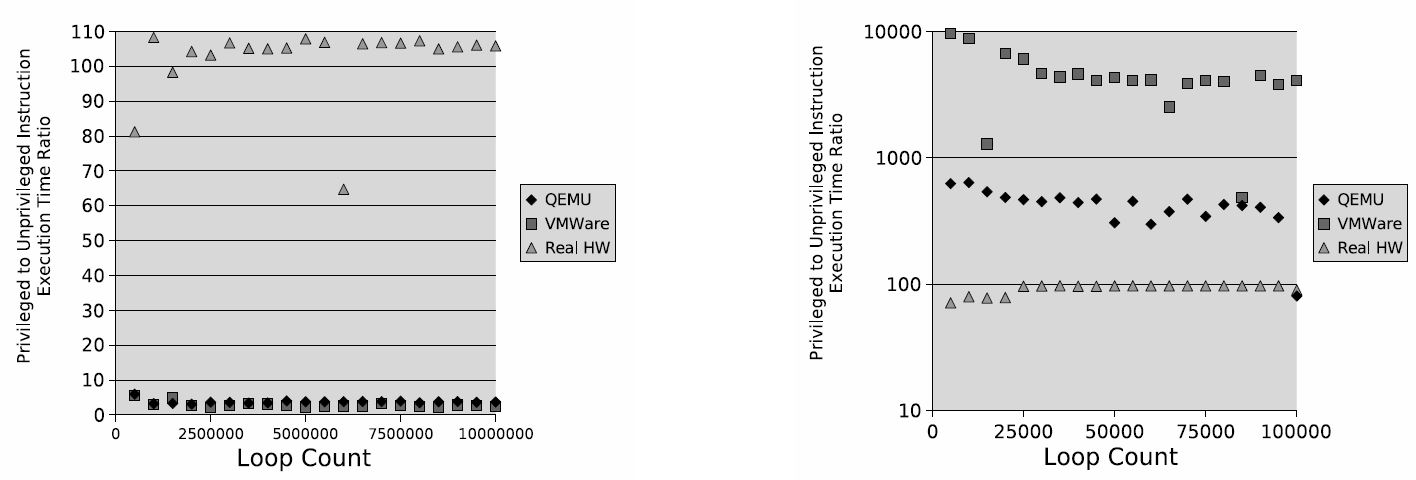
\includegraphics[width=\textwidth]{figure/comp_inst.jpg}
	\caption{Reading/Writing on CR0 (left) and CR3 (right)}
	\label{fig:comparison_of_instructions}
\end{figure*}

\subsubsection{Comparison of Instructions}
Even though a single performance score does not provide any meaningful clues, comparing the time taken between privileged instructions and unprivileged instructions can be useful to the VM detection mechanism. Raffetseder {\em et al.}~\cite{raffetseder2007} has used unprivileged instruction \textquotesingle s performance as a baseline and compare it privileged instruction \textquotesingle s to obtain relative performance number.
\begin{equation*}
Relative Performance = \frac{T_{privileged}}{T_{unprivileged}}
\end{equation*}
The insight is that real processors has to perform different tasks than simulated processors when handling privileged instructions. Thus it causes different relative performance results.  Raffetseder{\em et al.}~\cite{raffetseder2007} has conducted an experiment to prove the concept. A kernel module reads from a control register (CR0\footnote{contains various control flags} or CR3\footnote{When virtual addressing is enabled, CR3 register helps on virtual address to physical address translation}), then writes it back to where it came from. Raffetseder used processor\textquotesingle s time stamp counter (TSC) to measure the time elapsed to execute instructions. Figure~\ref{fig:comparison_of_instructions} shows the results. Real hardware showed poor relative performances when accessing CR0 but showed greater performance on CR3. Although Raffetseder did not explicitly explained why the results are different, it experiments showed a about difference in terms of 10 to 100 times between emulated and real environments. Thus, the difference is large enough to detect virtual environments.

\subsubsection{Mitigation of Comparison of Instructions} \label{sssec:mitigation_relative}
Raffetseder\textquotesingle s~\cite{raffetseder2007} experiments on comparison of instructions were done on software based emulation solutions (e.g. Qemu, VMware, etc.) which are buggy and fundamentally more limited than hardware solutions (e.g. Intel VT-x, AMD-V). Intel VT-x that runs on Xen hypervisor provides \texttt{TSC\_OFFSET} (Timestamp-Counter Scaling Offset) field additional to the regular  \texttt{TSC} field that is specifically design to skew the guest time upon clock cycle requests. When the guest guest queries for the \texttt{TSC} value, the hypervisor would return the difference between the \texttt{TSC} and \texttt{TSC\_OFFSET} as the clock cycle. Since the \texttt{TSC\_OFFSET} is under control of the hypervisor, sandboxing the malware on hardware based virtual environment should mitigate the relative performance difference vulnerability.

\subsubsection{Cached Instructions}
Caching lets the system hold on to recently executed functions in case they are needed again in near future. As a result, executing cached functions will consume less CPU cycles compared to the first time as shown on Figure~\ref{fig:cache_realhw} left. However, caching can be turned off on machines running on bare metal by making the processor enter the no-fill cache mode and flushing out all existing caches by using the WBINVD instruction. As a result, latter executions consume as much CPU cycles as the first run as shown on Figure~\ref{fig:cache_realhw} right.
However, it was shown that disabling caching is not properly supported on Qemu and VMware. Raffetseder{\em et al.}~\cite{raffetseder2007} has executed six independent test runs where each test run consists of five calls to one function. Both the Qemu (Figure~\ref{fig:cache_qemu}) and VMware (Figure~\ref{fig:cache_vmware}) had significant CPU cycle reduction after the first execution regardless of the caching preference.
Therefore, malware authors can take advantage of the fact the caching canno reallyt be turned off on virtual environments. If a malware obtain measurements similar to Figure~\ref{fig:cache_qemu} or Figure~\ref{fig:cache_vmware}, it should consider itself being in a sandbox and hide its malicious executions.
The malware authors can also take advantage of TLB flush to detect sandboxes. As mentioned in \ref{sssec:mitigation_relative}, software based solutions are very buggy and fundamentally limited to provide good virtualization, thus it is easy for malwares to detect them. For sandboxes running on top ofhardware assisted virtualization can trigger TLB flush to emulated caching being disabled. When a context switch is made from the guest to the hypervisor, the TLB is flushed to change the guest \textquotesingle s context to hypervisor \textquotesingle s context. Since TLB flush can be triggered by using non-privileged instructions \footnote{trapped down to the hypervisor and also available in the guest}, the time taken by an instruction can be calculated by running something like shown in figure~\ref{fig:cache_mitigation}. Upon calling non-privileged instructions that should cause TLB flushed multiple times, the time taken will decrease if TLB has not been flushed. However, the TLB has been flushed, then the time will increase. 

\subsubsection{Mitigation of Cached Instructions}
Controling low level CPU caching is very difficult due to 8 way set associative architecture. Thus, even just trying to fill up cache is not a easy job. There is no good solution known to prevent caching based VM detection in the resarch community. Theoratically, Address Space Identifier  (ASID) can control prevent flushing. However, it is also difficult to use it effectively on low level cache. 

\begin{figure}[h]
\begin{lstc}
; calc mean time before
loop:
	retsc
	;; test
	rdtsc

; flush tlb
cpuid

; check time after
rdtsc
;;test
rdtsc

; very different? 
cmp $before $after
\end{lstc}
\caption{\label{fig:cache_mitigation} Assembly code to measure the instruction meantime}
\end{figure}


\begin{figure*}[!t]
	\centering
	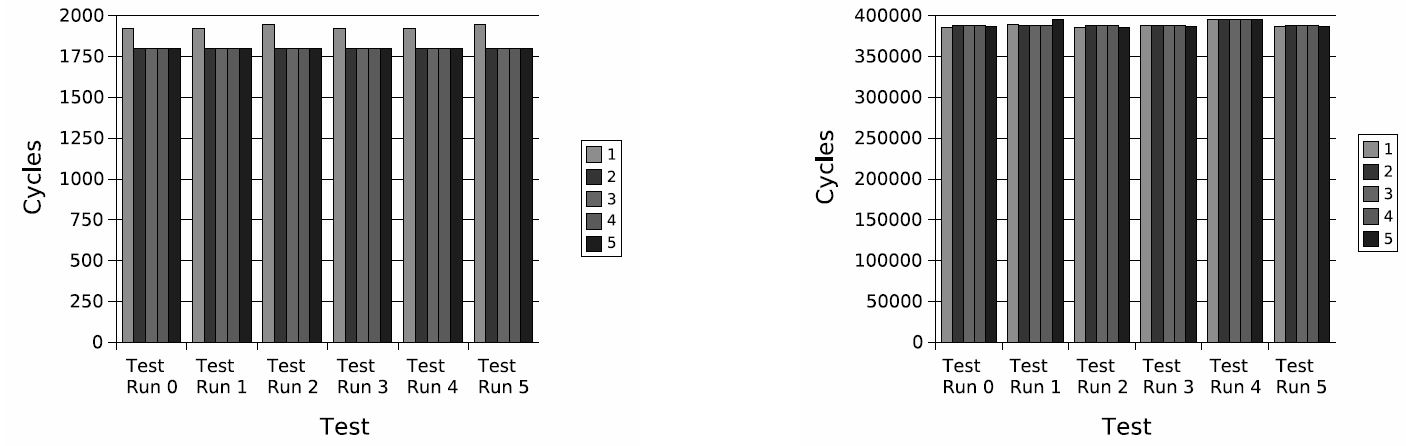
\includegraphics[width=\textwidth]{figure/realhw.jpg}
	\caption{Real hardware Cache On (left), Cache Off (right)}
	\label{fig:cache_realhw}
\end{figure*}

\begin{figure*}[!t]
	\centering
	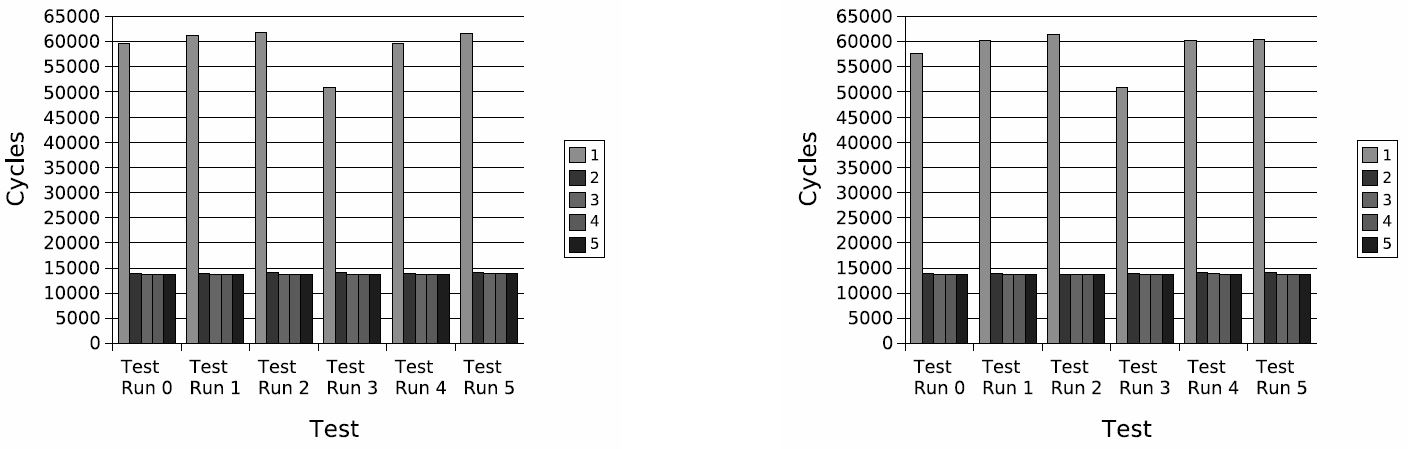
\includegraphics[width=\textwidth]{figure/qemu.jpg}
	\caption{Qemu On (left), Cache Off (right)}
	\label{fig:cache_qemu}
\end{figure*}

\begin{figure*}[!t]
	\centering
	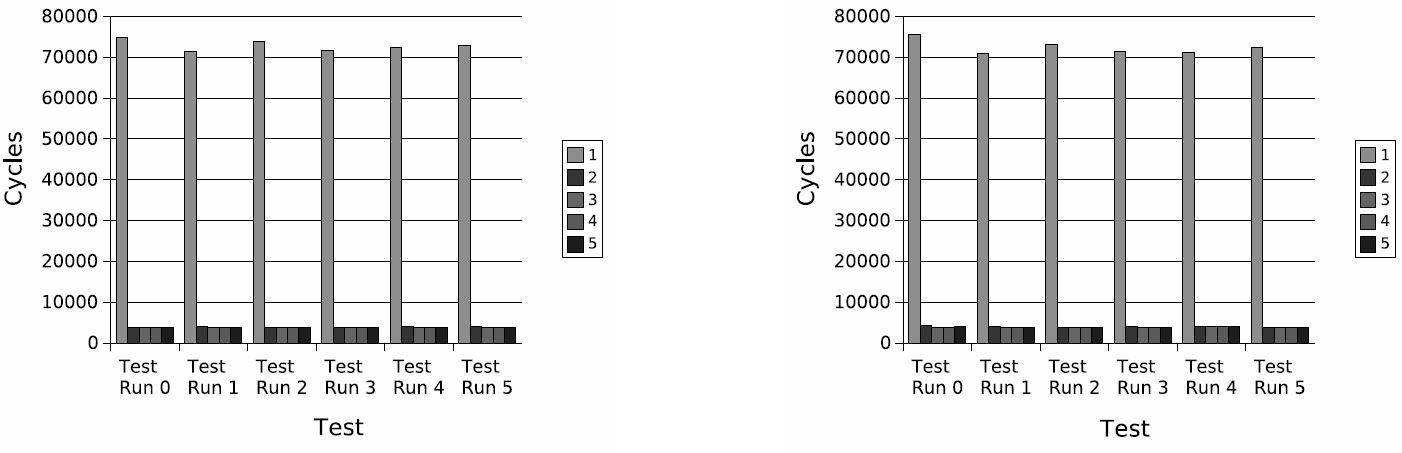
\includegraphics[width=\textwidth]{figure/vmware.jpg}
	\caption{VMware Cache On (left), Cache Off (right)}
	\label{fig:cache_vmware}
\end{figure*}

%%% Local Variables:
%%% mode: latex
%%% TeX-master: "../paper"
%%% End:


\vspace{8pt}
\section{Limitations}
\label{sec:limit}
Garfinkel {\em et al.}~\cite{garfinkel2007} believe that complete transparency
of VMM is infeasible and is contrary to the fundamental limitations of
virtualization technology. Regardless of the detection type, making the software
based virtualization transparent is infeasible due to countless bugs. On the
hardware-based type however, CPUID and CPU errata based methods are small enough to play the cat and mouse game where malware
authors find vulnerabilities and security professionals patch the vulnerable
instructions. For the timing based attacks, it is very difficult to prevent
relative comparison attacks and cache based attacks.
Detecting virtualization can also have benign use. Virtual Machine
Based Root-kits (VMBR) make AV software have to detect virtualization as
well~\cite{thompson, ferrie2007}. Examples are BluePill~\cite{bluepill} and
Vitriol~\cite{vitriol}, both using virtualization extensions (both Intel and
AMD). Therefore, the research community should be aware of the fact that
completly transparent VMs is a double-edged sword.m

%%% Local Variables:
%%% mode: latex
%%% TeX-master: "../paper"
%%% End:


\vspace{8pt}
\section{Conclusion}
\label{sec:conc}
Detecting virtualization can also have benign use. Virtual Machine Based Root-kits (VMBR) make AV software have to detect virtualization as well~\cite{thompson, ferrie2007}. Examples are BluePill~\cite{bluepill} and Vitriol~\cite{vitriol}, both using virtualization extensions (both Intel and AMD). Therefore, the research community should be aware of the fact that completly transparent VMs can also be a double-edged sword.

%%% Local Variables:
%%% mode: latex
%%% TeX-master: "../paper"
%%% End:


\vspace{10pt}
\bibliographystyle{unsrt}
{
\raggedright
\bibliography{publications}
}

\newpage
\section*{Appendix}
\label{sec:appendix}
\begin{figure}[h]
\begin{lstc}
#define CPUID_GETFEATURES 0x00000001
#define CPUID_FEAT_EDX_TSC (1 << 4)
...
__asm__ volatile ("cpuid" :
    "=a" (regs->rax),
    "=b" (regs->rbx),
    "=c" (regs->rcx),
    "=d" (regs->rdx)
    : "a" (CPUID_GETFEATURES), "c" (0));

tsc  = (regs->rdx & CPUID_FEAT_EDX_TSC);

if (!tsc) printf("detected ether!\n");
\end{lstc}
\caption{\label{fig:cpuid-tsc} Code snippet in C showing how to check for TSC
  support through the CPUID instruction.}
\end{figure}

\begin{figure*}[!t]
	\centering
	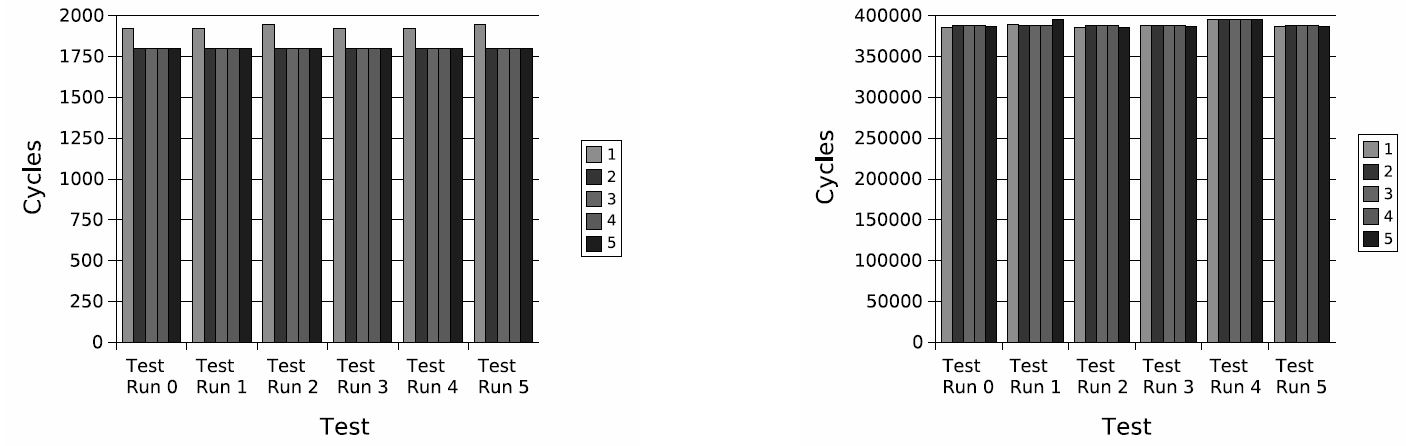
\includegraphics[width=\textwidth]{figure/realhw.jpg}
	\caption{Real hardware Cache On (left), Cache Off (right)}
	\label{fig:cache_realhw}
\end{figure*}

\begin{figure*}[!t]
	\centering
	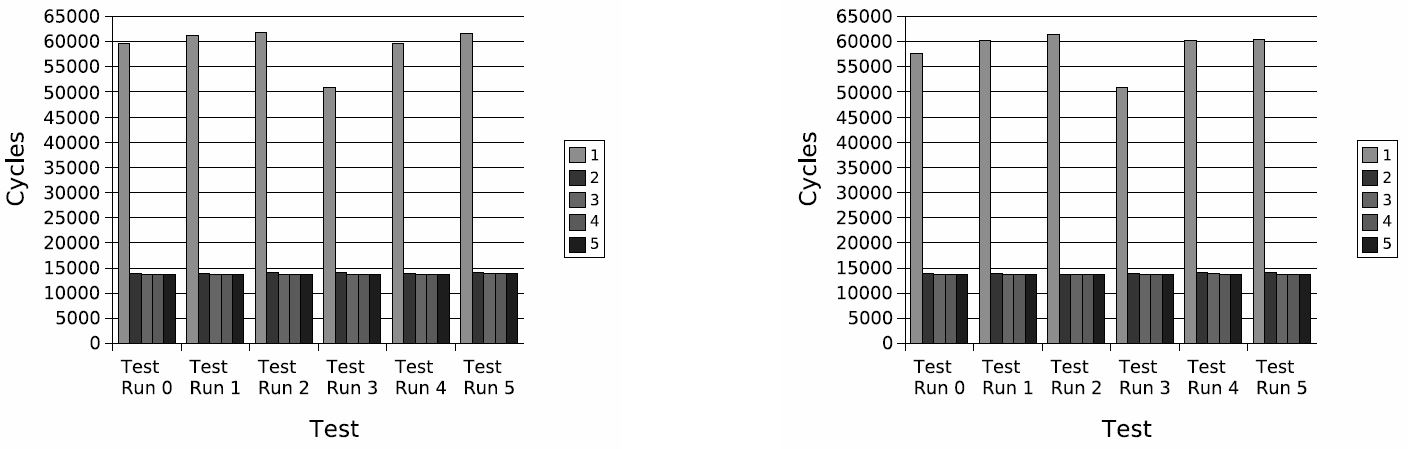
\includegraphics[width=\textwidth]{figure/qemu.jpg}
	\caption{Qemu On (left), Cache Off (right)}
	\label{fig:cache_qemu}
\end{figure*}

\begin{figure*}[!t]
	\centering
	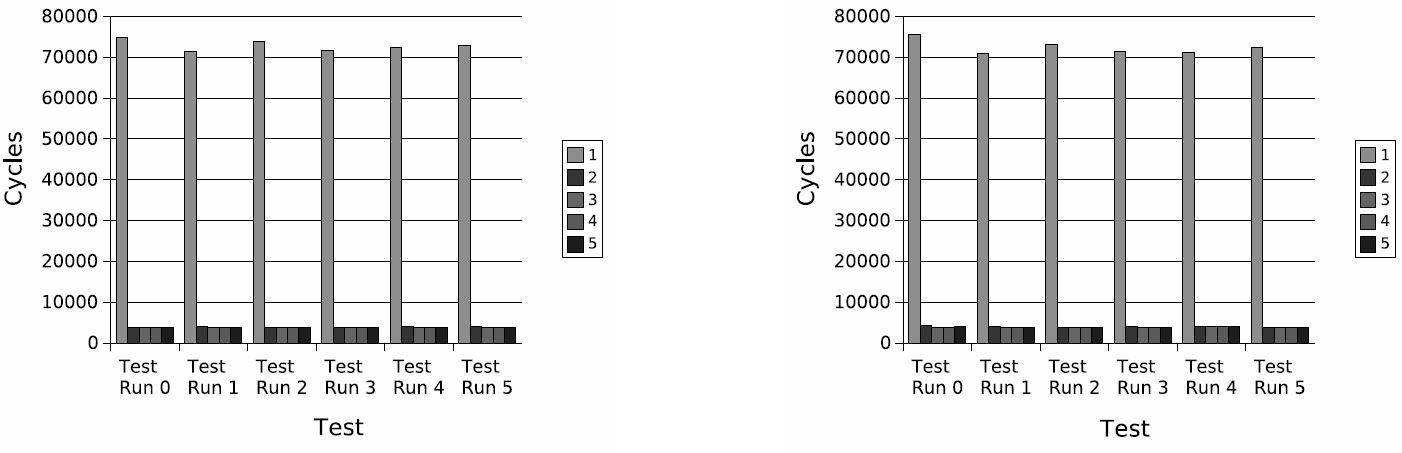
\includegraphics[width=\textwidth]{figure/vmware.jpg}
	\caption{VMware Cache On (left), Cache Off (right)}
	\label{fig:cache_vmware}
\end{figure*}

%%% Local Variables:
%%% mode: latex
%%% TeX-master: "../paper"
%%% End:


\end{document}
